\chapter{Data Acquisition and Software}
\label{chap:\currfilebase}


\section{Data acquistion}

The data acquisition system developed in this thesis is an open source Arduino based system consisting of multiple microcontrollers. All signal channels are transmitted to a central microcontroller before passing it to a computer that serves as visualization and analysis tool.

\begin{figure}[!htb]
    \centering
    \subcaptionbox{Without signal conditioning\label{sfig:dac_comp_simple}}
        {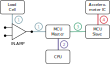
\includegraphics[scale=0.5]{\imgpath/dac/dac_components/dac_comp_simple}}
        \hfill
    \subcaptionbox{With signal conditioning and external \ac{ADC}\label{sfig:dac_comp_precond}}
        {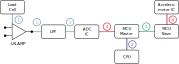
\includegraphics[scale=0.5]{\imgpath/dac/dac_components/dac_comp_precond}}
    \\[0.5em]
    \caption[DAC building blocks]{\ac{DAC}-system building blocks}
    \label{fig:dac_building_blocks}
\end{figure}

\begin{table}[!htb]
    \centering
    \def\linelabel#1#2{%
        \begin{tikzpicture}[%
            x=1em,y=1ex,
            baseline=(N.south),
            font={\fontsize{6pt}{6.2pt}\selectfont},
            ]%
            \draw[#1, line width=1pt] (0,1) -- (1,1) node [
                midway, above, yshift=1,
                circle, fill=white, draw=#1, line width=1pt,
                inner sep=2pt, minimum size=8pt, align=center,
                ] (N) {#2};
        \end{tikzpicture}
    }
    \footnotesize
		\begin{tabular}{c@{ :\hskip 0.5em}l}
            \toprule
            \multicolumn{2}{c}{Interfaces}\\
            \midrule
            \linelabel{WesMixL8qual0}{1} & Analog Signal\\
            \linelabel{WesMixL8qual3}{2} & \ac{USB}\\
            \linelabel{WesMixL8qual4}{3} & \ac{RS}-485\\
            \linelabel{WesMixL8qual6}{4} & \ac{SPI}\\
			\bottomrule
		\end{tabular}
    \normalsize
    \caption[Legend to DAC building blocks]{Legend to \figref{fig:dac_building_blocks}}
\end{table}


\subsection{Interfaces}

The interfaces are the connections and protocols between the different building blocks of the \ac{DAC} system. The interfaces are chosen based on the sensors used, and the expected data rate at the required cable length between each section. I.e.:

\begin{itemize}
    \item Between the analog \ac{LC} and the external \ac{ADC} in \figref{sfig:dac_comp_precond} and the \ac{MCU} integrated \ac{ADC}  in \figref{sfig:dac_comp_simple} respectively the signal transmission is analog.
    \item The register of the accelerometer \ac{IC} is accessed via \ac{SPI}
    \item The communication between \acs{MCU}s is rooted in \acs{RS}-485 differential transmission to accommodate for signal transmission over cable lengths greater than \SI{10}{\meters} and uses a specialized protocol to keep data packages as small as possible.
    \item Between the \ac{MCU} and the \ac{CPU} \ac{USB} transmitts data using the serial class of the Arduino software.
\end{itemize}


    output signal that must be amplified by an \ac{IN-AMP} to scale up the signal to the operating range of the consecutive components.

. to of smart sensor IC are predetermined. With \ac{SPI}Standard interfaces, determined by senor ic
MCU com based uart length -> differential transmission using the rs-485 protocol, introduces slave master com, only one slave can speak at a time

\subsection{Building Blocks}
mcus
arduino due,
tinsy, higher resolution
stm32

rs-485 converter

adcs

instrumentation amplifiers

\subsection{Dataflow}

All \acs{MCU}s operate sequentially.
The dataflow in \ac{MCU} must be sequential. For this reason all data passed to a central \ac{MCU}

In the case of multiple acceleroemeters 
multiple accelerometers, master requests for data in slave buffer cyclic, changes slave, limits of arduino library, 

\begin{figure}[!htb]
    \centering
    \includestandalone[width=0.8\linewidth]{\imgpath/software/data_flow/data_flow}
    \caption[Data flow]{Data flow between two MCU's and the CPU}
    \label{fig:data_flow}
\end{figure}
\subsubsection{MCU communication protocol}

The communication protocol between microcontrollers and between microcontroller and computer was developed for this project.
 
\begin{table}[!htb]
    \centering
    \includestandalone[scale=1]{\imgpath/software/mcu_com_protocol/mcu_com_protocol}
    \\[0.5em]
    \footnotesize
		\begin{tabular}{c@{ :\hskip 0.5em}l}
			\toprule
            \large{\textcolor{WesMixL8qual6}{<[}/\textcolor{WesMixL8qual6}{]>}} & Start-/End-bytes, represented as \ac{ASCII}\\
            \textcolor{WesMixL8qual0}{\large (reg)} & Registry/Address of the transmission\\
            \textcolor{WesMixL8qual4}{\large (\#Bytes)} & Number of bytes in transmission\\
            \textcolor{WesMixL8qual5}{\large (data)} & Data to transmit\\
			\bottomrule
		\end{tabular}
	\normalsize
    \caption[MCU communication protocol]{Protocol used to communicate between two MCU's and between MCU and computer}
    \label{tab:mcu_com_protocol}
\end{table}

\section{Software}

The software developed during this project is split into the Arduino software running on the \acs{MCU}s and a python based tool to receive and visualize the data via \ac{USB}.

The requirements to the software tools are:
\begin{enumerate}[label=m\arabic*]
    \item Read out accelerometer and \ac{LC} data at the maximum sample speed of the accelerometer \ac{IC}.
    \item Synchronize measurements timestamps
    \item Initialize measurement by hammer impulse
\end{enumerate}
    
\begin{enumerate}[label=w\arabic]
    \item Continuous real time output of measurement data
    \item Cache clearing
\end{enumerate}